\documentclass[twoside]{book}

% Packages required by doxygen
\usepackage{fixltx2e}
\usepackage{calc}
\usepackage{doxygen}
\usepackage[export]{adjustbox} % also loads graphicx
\usepackage{graphicx}
\usepackage[utf8]{inputenc}
\usepackage{makeidx}
\usepackage{multicol}
\usepackage{multirow}
\PassOptionsToPackage{warn}{textcomp}
\usepackage{textcomp}
\usepackage[nointegrals]{wasysym}
\usepackage[table]{xcolor}

% Font selection
\usepackage[T1]{fontenc}
\usepackage[scaled=.90]{helvet}
\usepackage{courier}
\usepackage{amssymb}
\usepackage{sectsty}
\renewcommand{\familydefault}{\sfdefault}
\allsectionsfont{%
  \fontseries{bc}\selectfont%
  \color{darkgray}%
}
\renewcommand{\DoxyLabelFont}{%
  \fontseries{bc}\selectfont%
  \color{darkgray}%
}
\newcommand{\+}{\discretionary{\mbox{\scriptsize$\hookleftarrow$}}{}{}}

% Page & text layout
\usepackage{geometry}
\geometry{%
  a4paper,%
  top=2.5cm,%
  bottom=2.5cm,%
  left=2.5cm,%
  right=2.5cm%
}
\tolerance=750
\hfuzz=15pt
\hbadness=750
\setlength{\emergencystretch}{15pt}
\setlength{\parindent}{0cm}
\setlength{\parskip}{3ex plus 2ex minus 2ex}
\makeatletter
\renewcommand{\paragraph}{%
  \@startsection{paragraph}{4}{0ex}{-1.0ex}{1.0ex}{%
    \normalfont\normalsize\bfseries\SS@parafont%
  }%
}
\renewcommand{\subparagraph}{%
  \@startsection{subparagraph}{5}{0ex}{-1.0ex}{1.0ex}{%
    \normalfont\normalsize\bfseries\SS@subparafont%
  }%
}
\makeatother

% Headers & footers
\usepackage{fancyhdr}
\pagestyle{fancyplain}
\fancyhead[LE]{\fancyplain{}{\bfseries\thepage}}
\fancyhead[CE]{\fancyplain{}{}}
\fancyhead[RE]{\fancyplain{}{\bfseries\leftmark}}
\fancyhead[LO]{\fancyplain{}{\bfseries\rightmark}}
\fancyhead[CO]{\fancyplain{}{}}
\fancyhead[RO]{\fancyplain{}{\bfseries\thepage}}
\fancyfoot[LE]{\fancyplain{}{}}
\fancyfoot[CE]{\fancyplain{}{}}
\fancyfoot[RE]{\fancyplain{}{\bfseries\scriptsize Generated by Doxygen }}
\fancyfoot[LO]{\fancyplain{}{\bfseries\scriptsize Generated by Doxygen }}
\fancyfoot[CO]{\fancyplain{}{}}
\fancyfoot[RO]{\fancyplain{}{}}
\renewcommand{\footrulewidth}{0.4pt}
\renewcommand{\chaptermark}[1]{%
  \markboth{#1}{}%
}
\renewcommand{\sectionmark}[1]{%
  \markright{\thesection\ #1}%
}

% Indices & bibliography
\usepackage{natbib}
\usepackage[titles]{tocloft}
\setcounter{tocdepth}{3}
\setcounter{secnumdepth}{5}
\makeindex

% Hyperlinks (required, but should be loaded last)
\usepackage{ifpdf}
\ifpdf
  \usepackage[pdftex,pagebackref=true]{hyperref}
\else
  \usepackage[ps2pdf,pagebackref=true]{hyperref}
\fi
\hypersetup{%
  colorlinks=true,%
  linkcolor=blue,%
  citecolor=blue,%
  unicode%
}

% Custom commands
\newcommand{\clearemptydoublepage}{%
  \newpage{\pagestyle{empty}\cleardoublepage}%
}

\usepackage{caption}
\captionsetup{labelsep=space,justification=centering,font={bf},singlelinecheck=off,skip=4pt,position=top}

%===== C O N T E N T S =====

\begin{document}

% Titlepage & ToC
\hypersetup{pageanchor=false,
             bookmarksnumbered=true,
             pdfencoding=unicode
            }
\pagenumbering{alph}
\begin{titlepage}
\vspace*{7cm}
\begin{center}%
{\Large My Project }\\
\vspace*{1cm}
{\large Generated by Doxygen 1.8.13}\\
\end{center}
\end{titlepage}
\clearemptydoublepage
\pagenumbering{roman}
\tableofcontents
\clearemptydoublepage
\pagenumbering{arabic}
\hypersetup{pageanchor=true}

%--- Begin generated contents ---
\chapter{Namespace Index}
\section{Namespace List}
Here is a list of all namespaces with brief descriptions\+:\begin{DoxyCompactList}
\item\contentsline{section}{\hyperlink{namespacesensor}{sensor} }{\pageref{namespacesensor}}{}
\end{DoxyCompactList}

\chapter{Hierarchical Index}
\section{Class Hierarchy}
This inheritance list is sorted roughly, but not completely, alphabetically\+:\begin{DoxyCompactList}
\item \contentsline{section}{Sensor}{\pageref{class_sensor}}{}
\begin{DoxyCompactList}
\item \contentsline{section}{sensor\+:\+:Accelerometer}{\pageref{classsensor_1_1_accelerometer}}{}
\item \contentsline{section}{sensor\+:\+:G\+PS}{\pageref{classsensor_1_1_g_p_s}}{}
\item \contentsline{section}{sensor\+:\+:Magnetometer}{\pageref{classsensor_1_1_magnetometer}}{}
\end{DoxyCompactList}
\end{DoxyCompactList}

\chapter{Class Index}
\section{Class List}
Here are the classes, structs, unions and interfaces with brief descriptions\+:\begin{DoxyCompactList}
\item\contentsline{section}{\hyperlink{classsensor_1_1_accelerometer}{sensor\+::\+Accelerometer} }{\pageref{classsensor_1_1_accelerometer}}{}
\item\contentsline{section}{\hyperlink{classsensor_1_1_g_p_s}{sensor\+::\+G\+PS} }{\pageref{classsensor_1_1_g_p_s}}{}
\item\contentsline{section}{\hyperlink{classsensor_1_1_magnetometer}{sensor\+::\+Magnetometer} }{\pageref{classsensor_1_1_magnetometer}}{}
\item\contentsline{section}{\hyperlink{class_sensor}{Sensor} }{\pageref{class_sensor}}{}
\end{DoxyCompactList}

\chapter{File Index}
\section{File List}
Here is a list of all files with brief descriptions\+:\begin{DoxyCompactList}
\item\contentsline{section}{include/\hyperlink{accelerometer_8h}{accelerometer.\+h} }{\pageref{accelerometer_8h}}{}
\item\contentsline{section}{include/\hyperlink{functions_8h}{functions.\+h} }{\pageref{functions_8h}}{}
\item\contentsline{section}{include/\hyperlink{gps_8h}{gps.\+h} }{\pageref{gps_8h}}{}
\item\contentsline{section}{include/\hyperlink{magnetometer_8h}{magnetometer.\+h} }{\pageref{magnetometer_8h}}{}
\item\contentsline{section}{include/\hyperlink{sensor_8h}{sensor.\+h} }{\pageref{sensor_8h}}{}
\item\contentsline{section}{src/\hyperlink{accelerometer_8cpp}{accelerometer.\+cpp} }{\pageref{accelerometer_8cpp}}{}
\item\contentsline{section}{src/\hyperlink{functions_8cpp}{functions.\+cpp} }{\pageref{functions_8cpp}}{}
\item\contentsline{section}{src/\hyperlink{gps_8cpp}{gps.\+cpp} }{\pageref{gps_8cpp}}{}
\item\contentsline{section}{src/\hyperlink{magnetometer_8cpp}{magnetometer.\+cpp} }{\pageref{magnetometer_8cpp}}{}
\item\contentsline{section}{src/\hyperlink{main_8cpp}{main.\+cpp} }{\pageref{main_8cpp}}{}
\item\contentsline{section}{src/\hyperlink{sensor_8cpp}{sensor.\+cpp} }{\pageref{sensor_8cpp}}{}
\end{DoxyCompactList}

\chapter{Namespace Documentation}
\hypertarget{namespacesensor}{}\section{sensor Namespace Reference}
\label{namespacesensor}\index{sensor@{sensor}}
\subsection*{Classes}
\begin{DoxyCompactItemize}
\item 
class \hyperlink{classsensor_1_1_accelerometer}{Accelerometer}
\item 
class \hyperlink{classsensor_1_1_g_p_s}{G\+PS}
\item 
class \hyperlink{classsensor_1_1_magnetometer}{Magnetometer}
\end{DoxyCompactItemize}
\subsection*{Functions}
\begin{DoxyCompactItemize}
\item 
std\+::vector$<$ double $>$ \hyperlink{namespacesensor_a8d403ba02d81030a8c321487632d6dfd}{Roll\+Pitch\+Yaw} (\hyperlink{classsensor_1_1_accelerometer}{Accelerometer} \&obj\+\_\+acc, \hyperlink{classsensor_1_1_magnetometer}{Magnetometer} \&obj\+\_\+mag)
\end{DoxyCompactItemize}


\subsection{Function Documentation}
\mbox{\Hypertarget{namespacesensor_a8d403ba02d81030a8c321487632d6dfd}\label{namespacesensor_a8d403ba02d81030a8c321487632d6dfd}} 
\index{sensor@{sensor}!Roll\+Pitch\+Yaw@{Roll\+Pitch\+Yaw}}
\index{Roll\+Pitch\+Yaw@{Roll\+Pitch\+Yaw}!sensor@{sensor}}
\subsubsection{\texorpdfstring{Roll\+Pitch\+Yaw()}{RollPitchYaw()}}
{\footnotesize\ttfamily std\+::vector$<$ double $>$ sensor\+::\+Roll\+Pitch\+Yaw (\begin{DoxyParamCaption}\item[{\hyperlink{classsensor_1_1_accelerometer}{Accelerometer} \&}]{obj\+\_\+acc,  }\item[{\hyperlink{classsensor_1_1_magnetometer}{Magnetometer} \&}]{obj\+\_\+mag }\end{DoxyParamCaption})}



Definition at line 4 of file functions.\+cpp.


\chapter{Class Documentation}
\hypertarget{classsensor_1_1_accelerometer}{}\section{sensor\+:\+:Accelerometer Class Reference}
\label{classsensor_1_1_accelerometer}\index{sensor\+::\+Accelerometer@{sensor\+::\+Accelerometer}}


{\ttfamily \#include $<$accelerometer.\+h$>$}



Inheritance diagram for sensor\+:\+:Accelerometer\+:\nopagebreak
\begin{figure}[H]
\begin{center}
\leavevmode
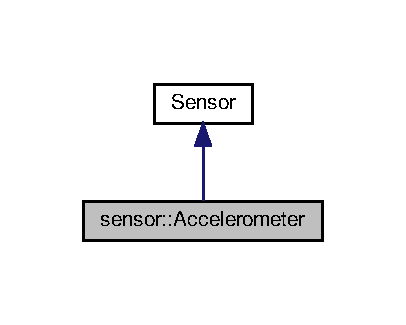
\includegraphics[width=195pt]{classsensor_1_1_accelerometer__inherit__graph}
\end{center}
\end{figure}


Collaboration diagram for sensor\+:\+:Accelerometer\+:\nopagebreak
\begin{figure}[H]
\begin{center}
\leavevmode
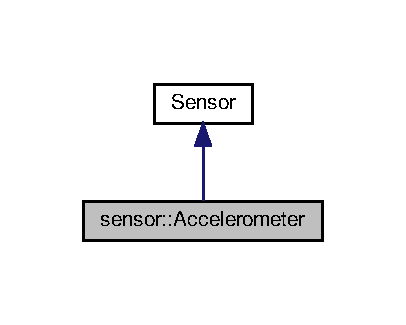
\includegraphics[width=195pt]{classsensor_1_1_accelerometer__coll__graph}
\end{center}
\end{figure}
\subsection*{Public Member Functions}
\begin{DoxyCompactItemize}
\item 
\hyperlink{classsensor_1_1_accelerometer_a6615c08a2b256bd1e1f2ddc09e9337cb}{Accelerometer} ()
\item 
\hyperlink{classsensor_1_1_accelerometer_a375d0a6727812144705808e10039cba2}{Accelerometer} (double x, double y, double z)
\item 
\hyperlink{classsensor_1_1_accelerometer_a03b06044198fcb5c39f9b83c471c5fd2}{$\sim$\+Accelerometer} ()
\item 
std\+::vector$<$ double $>$ \hyperlink{classsensor_1_1_accelerometer_a53257e59c7db9c75f3df41039d5b5b6d}{linear\+\_\+acceleration} (double gyro\+\_\+yaw, double gyro\+\_\+pitch, double gyro\+\_\+roll)
\item 
virtual void \hyperlink{classsensor_1_1_accelerometer_a172c1bfe5d20071d5f3542a717797afa}{print\+\_\+raw} ()
\item 
double \hyperlink{classsensor_1_1_accelerometer_afd2bf373d1142b305cc16c9020ae01e8}{pitch} ()
\item 
double \hyperlink{classsensor_1_1_accelerometer_a63e28e79c1b08471c86f163033b04c5d}{roll} ()
\end{DoxyCompactItemize}
\subsection*{Friends}
\begin{DoxyCompactItemize}
\item 
std\+::vector$<$ double $>$ \hyperlink{classsensor_1_1_accelerometer_af6581f59b9f71cabfa36a46d177deb5f}{Roll\+Pitch\+Yaw} (\hyperlink{classsensor_1_1_accelerometer}{Accelerometer} \&, \hyperlink{classsensor_1_1_magnetometer}{Magnetometer} \&)
\end{DoxyCompactItemize}
\subsection*{Additional Inherited Members}


\subsection{Detailed Description}


Definition at line 15 of file accelerometer.\+h.



\subsection{Constructor \& Destructor Documentation}
\mbox{\Hypertarget{classsensor_1_1_accelerometer_a6615c08a2b256bd1e1f2ddc09e9337cb}\label{classsensor_1_1_accelerometer_a6615c08a2b256bd1e1f2ddc09e9337cb}} 
\index{sensor\+::\+Accelerometer@{sensor\+::\+Accelerometer}!Accelerometer@{Accelerometer}}
\index{Accelerometer@{Accelerometer}!sensor\+::\+Accelerometer@{sensor\+::\+Accelerometer}}
\subsubsection{\texorpdfstring{Accelerometer()}{Accelerometer()}\hspace{0.1cm}{\footnotesize\ttfamily [1/2]}}
{\footnotesize\ttfamily sensor\+::\+Accelerometer\+::\+Accelerometer (\begin{DoxyParamCaption}{ }\end{DoxyParamCaption})}



Definition at line 5 of file accelerometer.\+cpp.

\mbox{\Hypertarget{classsensor_1_1_accelerometer_a375d0a6727812144705808e10039cba2}\label{classsensor_1_1_accelerometer_a375d0a6727812144705808e10039cba2}} 
\index{sensor\+::\+Accelerometer@{sensor\+::\+Accelerometer}!Accelerometer@{Accelerometer}}
\index{Accelerometer@{Accelerometer}!sensor\+::\+Accelerometer@{sensor\+::\+Accelerometer}}
\subsubsection{\texorpdfstring{Accelerometer()}{Accelerometer()}\hspace{0.1cm}{\footnotesize\ttfamily [2/2]}}
{\footnotesize\ttfamily sensor\+::\+Accelerometer\+::\+Accelerometer (\begin{DoxyParamCaption}\item[{double}]{x,  }\item[{double}]{y,  }\item[{double}]{z }\end{DoxyParamCaption})}



Definition at line 8 of file accelerometer.\+cpp.

\mbox{\Hypertarget{classsensor_1_1_accelerometer_a03b06044198fcb5c39f9b83c471c5fd2}\label{classsensor_1_1_accelerometer_a03b06044198fcb5c39f9b83c471c5fd2}} 
\index{sensor\+::\+Accelerometer@{sensor\+::\+Accelerometer}!````~Accelerometer@{$\sim$\+Accelerometer}}
\index{````~Accelerometer@{$\sim$\+Accelerometer}!sensor\+::\+Accelerometer@{sensor\+::\+Accelerometer}}
\subsubsection{\texorpdfstring{$\sim$\+Accelerometer()}{~Accelerometer()}}
{\footnotesize\ttfamily sensor\+::\+Accelerometer\+::$\sim$\+Accelerometer (\begin{DoxyParamCaption}{ }\end{DoxyParamCaption})}



Definition at line 11 of file accelerometer.\+cpp.



\subsection{Member Function Documentation}
\mbox{\Hypertarget{classsensor_1_1_accelerometer_a53257e59c7db9c75f3df41039d5b5b6d}\label{classsensor_1_1_accelerometer_a53257e59c7db9c75f3df41039d5b5b6d}} 
\index{sensor\+::\+Accelerometer@{sensor\+::\+Accelerometer}!linear\+\_\+acceleration@{linear\+\_\+acceleration}}
\index{linear\+\_\+acceleration@{linear\+\_\+acceleration}!sensor\+::\+Accelerometer@{sensor\+::\+Accelerometer}}
\subsubsection{\texorpdfstring{linear\+\_\+acceleration()}{linear\_acceleration()}}
{\footnotesize\ttfamily std\+::vector$<$double$>$ sensor\+::\+Accelerometer\+::linear\+\_\+acceleration (\begin{DoxyParamCaption}\item[{double}]{gyro\+\_\+yaw,  }\item[{double}]{gyro\+\_\+pitch,  }\item[{double}]{gyro\+\_\+roll }\end{DoxyParamCaption})}

\mbox{\Hypertarget{classsensor_1_1_accelerometer_afd2bf373d1142b305cc16c9020ae01e8}\label{classsensor_1_1_accelerometer_afd2bf373d1142b305cc16c9020ae01e8}} 
\index{sensor\+::\+Accelerometer@{sensor\+::\+Accelerometer}!pitch@{pitch}}
\index{pitch@{pitch}!sensor\+::\+Accelerometer@{sensor\+::\+Accelerometer}}
\subsubsection{\texorpdfstring{pitch()}{pitch()}}
{\footnotesize\ttfamily double sensor\+::\+Accelerometer\+::pitch (\begin{DoxyParamCaption}{ }\end{DoxyParamCaption})}



Definition at line 43 of file accelerometer.\+cpp.

\mbox{\Hypertarget{classsensor_1_1_accelerometer_a172c1bfe5d20071d5f3542a717797afa}\label{classsensor_1_1_accelerometer_a172c1bfe5d20071d5f3542a717797afa}} 
\index{sensor\+::\+Accelerometer@{sensor\+::\+Accelerometer}!print\+\_\+raw@{print\+\_\+raw}}
\index{print\+\_\+raw@{print\+\_\+raw}!sensor\+::\+Accelerometer@{sensor\+::\+Accelerometer}}
\subsubsection{\texorpdfstring{print\+\_\+raw()}{print\_raw()}}
{\footnotesize\ttfamily void sensor\+::\+Accelerometer\+::print\+\_\+raw (\begin{DoxyParamCaption}{ }\end{DoxyParamCaption})\hspace{0.3cm}{\ttfamily [virtual]}}



Reimplemented from \hyperlink{class_sensor_a6f16371eb71419f49ea1363ca81d0755}{Sensor}.



Definition at line 36 of file accelerometer.\+cpp.

\mbox{\Hypertarget{classsensor_1_1_accelerometer_a63e28e79c1b08471c86f163033b04c5d}\label{classsensor_1_1_accelerometer_a63e28e79c1b08471c86f163033b04c5d}} 
\index{sensor\+::\+Accelerometer@{sensor\+::\+Accelerometer}!roll@{roll}}
\index{roll@{roll}!sensor\+::\+Accelerometer@{sensor\+::\+Accelerometer}}
\subsubsection{\texorpdfstring{roll()}{roll()}}
{\footnotesize\ttfamily double sensor\+::\+Accelerometer\+::roll (\begin{DoxyParamCaption}{ }\end{DoxyParamCaption})}



Definition at line 52 of file accelerometer.\+cpp.



\subsection{Friends And Related Function Documentation}
\mbox{\Hypertarget{classsensor_1_1_accelerometer_af6581f59b9f71cabfa36a46d177deb5f}\label{classsensor_1_1_accelerometer_af6581f59b9f71cabfa36a46d177deb5f}} 
\index{sensor\+::\+Accelerometer@{sensor\+::\+Accelerometer}!Roll\+Pitch\+Yaw@{Roll\+Pitch\+Yaw}}
\index{Roll\+Pitch\+Yaw@{Roll\+Pitch\+Yaw}!sensor\+::\+Accelerometer@{sensor\+::\+Accelerometer}}
\subsubsection{\texorpdfstring{Roll\+Pitch\+Yaw}{RollPitchYaw}}
{\footnotesize\ttfamily std\+::vector$<$double$>$ Roll\+Pitch\+Yaw (\begin{DoxyParamCaption}\item[{\hyperlink{classsensor_1_1_accelerometer}{Accelerometer} \&}]{obj\+\_\+acc,  }\item[{\hyperlink{classsensor_1_1_magnetometer}{Magnetometer} \&}]{obj\+\_\+mag }\end{DoxyParamCaption})\hspace{0.3cm}{\ttfamily [friend]}}



Definition at line 4 of file functions.\+cpp.



The documentation for this class was generated from the following files\+:\begin{DoxyCompactItemize}
\item 
include/\hyperlink{accelerometer_8h}{accelerometer.\+h}\item 
src/\hyperlink{accelerometer_8cpp}{accelerometer.\+cpp}\end{DoxyCompactItemize}

\hypertarget{classsensor_1_1_g_p_s}{}\section{sensor\+:\+:G\+PS Class Reference}
\label{classsensor_1_1_g_p_s}\index{sensor\+::\+G\+PS@{sensor\+::\+G\+PS}}


{\ttfamily \#include $<$gps.\+h$>$}



Inheritance diagram for sensor\+:\+:G\+PS\+:\nopagebreak
\begin{figure}[H]
\begin{center}
\leavevmode
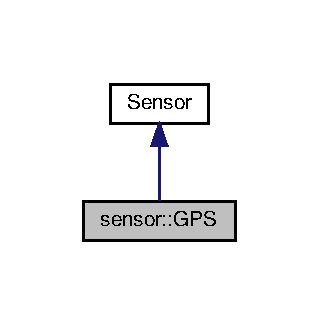
\includegraphics[width=153pt]{classsensor_1_1_g_p_s__inherit__graph}
\end{center}
\end{figure}


Collaboration diagram for sensor\+:\+:G\+PS\+:\nopagebreak
\begin{figure}[H]
\begin{center}
\leavevmode
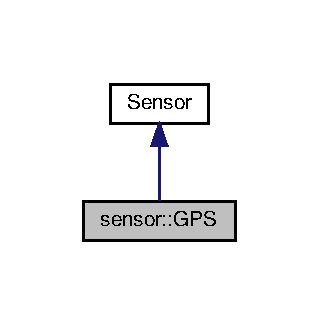
\includegraphics[width=153pt]{classsensor_1_1_g_p_s__coll__graph}
\end{center}
\end{figure}
\subsection*{Public Member Functions}
\begin{DoxyCompactItemize}
\item 
\hyperlink{classsensor_1_1_g_p_s_aee655f2d2f29485e622e75a38d15420c}{G\+PS} ()
\item 
\hyperlink{classsensor_1_1_g_p_s_a14837a509a3f16ebdd2f2ba5088f9b3f}{G\+PS} (std\+::string latitude, std\+::string longitude)
\item 
\hyperlink{classsensor_1_1_g_p_s_a40c60af10a932120408155ca430cbe34}{$\sim$\+G\+PS} ()
\item 
double \hyperlink{classsensor_1_1_g_p_s_a5d2f338838b59c6e980ff96bf5bc8087}{operator-\/} (\hyperlink{classsensor_1_1_g_p_s}{G\+PS} \&ref)
\item 
virtual void \hyperlink{classsensor_1_1_g_p_s_a8b0dfe608735ccca47bae8e9a41e1298}{print\+\_\+raw} ()
\end{DoxyCompactItemize}
\subsection*{Additional Inherited Members}


\subsection{Detailed Description}


Definition at line 13 of file gps.\+h.



\subsection{Constructor \& Destructor Documentation}
\mbox{\Hypertarget{classsensor_1_1_g_p_s_aee655f2d2f29485e622e75a38d15420c}\label{classsensor_1_1_g_p_s_aee655f2d2f29485e622e75a38d15420c}} 
\index{sensor\+::\+G\+PS@{sensor\+::\+G\+PS}!G\+PS@{G\+PS}}
\index{G\+PS@{G\+PS}!sensor\+::\+G\+PS@{sensor\+::\+G\+PS}}
\subsubsection{\texorpdfstring{G\+P\+S()}{GPS()}\hspace{0.1cm}{\footnotesize\ttfamily [1/2]}}
{\footnotesize\ttfamily sensor\+::\+G\+P\+S\+::\+G\+PS (\begin{DoxyParamCaption}{ }\end{DoxyParamCaption})}



Definition at line 25 of file gps.\+cpp.

\mbox{\Hypertarget{classsensor_1_1_g_p_s_a14837a509a3f16ebdd2f2ba5088f9b3f}\label{classsensor_1_1_g_p_s_a14837a509a3f16ebdd2f2ba5088f9b3f}} 
\index{sensor\+::\+G\+PS@{sensor\+::\+G\+PS}!G\+PS@{G\+PS}}
\index{G\+PS@{G\+PS}!sensor\+::\+G\+PS@{sensor\+::\+G\+PS}}
\subsubsection{\texorpdfstring{G\+P\+S()}{GPS()}\hspace{0.1cm}{\footnotesize\ttfamily [2/2]}}
{\footnotesize\ttfamily sensor\+::\+G\+P\+S\+::\+G\+PS (\begin{DoxyParamCaption}\item[{std\+::string}]{latitude,  }\item[{std\+::string}]{longitude }\end{DoxyParamCaption})}



Definition at line 27 of file gps.\+cpp.

\mbox{\Hypertarget{classsensor_1_1_g_p_s_a40c60af10a932120408155ca430cbe34}\label{classsensor_1_1_g_p_s_a40c60af10a932120408155ca430cbe34}} 
\index{sensor\+::\+G\+PS@{sensor\+::\+G\+PS}!````~G\+PS@{$\sim$\+G\+PS}}
\index{````~G\+PS@{$\sim$\+G\+PS}!sensor\+::\+G\+PS@{sensor\+::\+G\+PS}}
\subsubsection{\texorpdfstring{$\sim$\+G\+P\+S()}{~GPS()}}
{\footnotesize\ttfamily sensor\+::\+G\+P\+S\+::$\sim$\+G\+PS (\begin{DoxyParamCaption}{ }\end{DoxyParamCaption})}



Definition at line 32 of file gps.\+cpp.



\subsection{Member Function Documentation}
\mbox{\Hypertarget{classsensor_1_1_g_p_s_a5d2f338838b59c6e980ff96bf5bc8087}\label{classsensor_1_1_g_p_s_a5d2f338838b59c6e980ff96bf5bc8087}} 
\index{sensor\+::\+G\+PS@{sensor\+::\+G\+PS}!operator-\/@{operator-\/}}
\index{operator-\/@{operator-\/}!sensor\+::\+G\+PS@{sensor\+::\+G\+PS}}
\subsubsection{\texorpdfstring{operator-\/()}{operator-()}}
{\footnotesize\ttfamily double sensor\+::\+G\+P\+S\+::operator-\/ (\begin{DoxyParamCaption}\item[{\hyperlink{classsensor_1_1_g_p_s}{G\+PS} \&}]{ref }\end{DoxyParamCaption})}



Definition at line 34 of file gps.\+cpp.

\mbox{\Hypertarget{classsensor_1_1_g_p_s_a8b0dfe608735ccca47bae8e9a41e1298}\label{classsensor_1_1_g_p_s_a8b0dfe608735ccca47bae8e9a41e1298}} 
\index{sensor\+::\+G\+PS@{sensor\+::\+G\+PS}!print\+\_\+raw@{print\+\_\+raw}}
\index{print\+\_\+raw@{print\+\_\+raw}!sensor\+::\+G\+PS@{sensor\+::\+G\+PS}}
\subsubsection{\texorpdfstring{print\+\_\+raw()}{print\_raw()}}
{\footnotesize\ttfamily void sensor\+::\+G\+P\+S\+::print\+\_\+raw (\begin{DoxyParamCaption}{ }\end{DoxyParamCaption})\hspace{0.3cm}{\ttfamily [virtual]}}



Reimplemented from \hyperlink{class_sensor_a6f16371eb71419f49ea1363ca81d0755}{Sensor}.



Definition at line 47 of file gps.\+cpp.



The documentation for this class was generated from the following files\+:\begin{DoxyCompactItemize}
\item 
include/\hyperlink{gps_8h}{gps.\+h}\item 
src/\hyperlink{gps_8cpp}{gps.\+cpp}\end{DoxyCompactItemize}

\hypertarget{classsensor_1_1_magnetometer}{}\section{sensor\+:\+:Magnetometer Class Reference}
\label{classsensor_1_1_magnetometer}\index{sensor\+::\+Magnetometer@{sensor\+::\+Magnetometer}}


{\ttfamily \#include $<$magnetometer.\+h$>$}



Inheritance diagram for sensor\+:\+:Magnetometer\+:\nopagebreak
\begin{figure}[H]
\begin{center}
\leavevmode
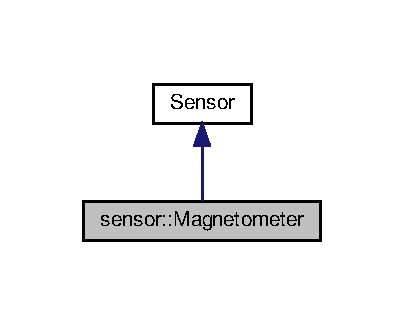
\includegraphics[width=194pt]{classsensor_1_1_magnetometer__inherit__graph}
\end{center}
\end{figure}


Collaboration diagram for sensor\+:\+:Magnetometer\+:\nopagebreak
\begin{figure}[H]
\begin{center}
\leavevmode
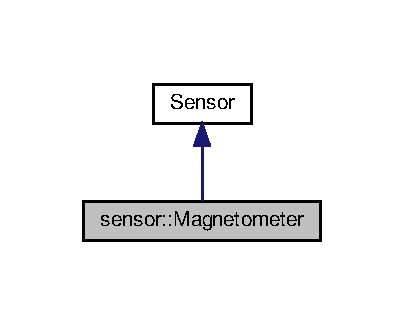
\includegraphics[width=194pt]{classsensor_1_1_magnetometer__coll__graph}
\end{center}
\end{figure}
\subsection*{Public Member Functions}
\begin{DoxyCompactItemize}
\item 
\hyperlink{classsensor_1_1_magnetometer_a09d5d8674a21e70460745081ac759d87}{Magnetometer} ()
\item 
\hyperlink{classsensor_1_1_magnetometer_a30b9846b3bbecf844e10845f47ff0bf5}{Magnetometer} (double x, double y, double z)
\item 
\hyperlink{classsensor_1_1_magnetometer_acaebbf476faf2f2e029e9d4e5d1ff896}{$\sim$\+Magnetometer} ()
\item 
virtual void \hyperlink{classsensor_1_1_magnetometer_a808eda46aabd080426c909563da0f425}{print\+\_\+raw} ()
\end{DoxyCompactItemize}
\subsection*{Friends}
\begin{DoxyCompactItemize}
\item 
std\+::vector$<$ double $>$ \hyperlink{classsensor_1_1_magnetometer_af6581f59b9f71cabfa36a46d177deb5f}{Roll\+Pitch\+Yaw} (\hyperlink{classsensor_1_1_accelerometer}{Accelerometer} \&, \hyperlink{classsensor_1_1_magnetometer}{Magnetometer} \&)
\end{DoxyCompactItemize}
\subsection*{Additional Inherited Members}


\subsection{Detailed Description}


Definition at line 13 of file magnetometer.\+h.



\subsection{Constructor \& Destructor Documentation}
\mbox{\Hypertarget{classsensor_1_1_magnetometer_a09d5d8674a21e70460745081ac759d87}\label{classsensor_1_1_magnetometer_a09d5d8674a21e70460745081ac759d87}} 
\index{sensor\+::\+Magnetometer@{sensor\+::\+Magnetometer}!Magnetometer@{Magnetometer}}
\index{Magnetometer@{Magnetometer}!sensor\+::\+Magnetometer@{sensor\+::\+Magnetometer}}
\subsubsection{\texorpdfstring{Magnetometer()}{Magnetometer()}\hspace{0.1cm}{\footnotesize\ttfamily [1/2]}}
{\footnotesize\ttfamily sensor\+::\+Magnetometer\+::\+Magnetometer (\begin{DoxyParamCaption}{ }\end{DoxyParamCaption})}



Definition at line 4 of file magnetometer.\+cpp.

\mbox{\Hypertarget{classsensor_1_1_magnetometer_a30b9846b3bbecf844e10845f47ff0bf5}\label{classsensor_1_1_magnetometer_a30b9846b3bbecf844e10845f47ff0bf5}} 
\index{sensor\+::\+Magnetometer@{sensor\+::\+Magnetometer}!Magnetometer@{Magnetometer}}
\index{Magnetometer@{Magnetometer}!sensor\+::\+Magnetometer@{sensor\+::\+Magnetometer}}
\subsubsection{\texorpdfstring{Magnetometer()}{Magnetometer()}\hspace{0.1cm}{\footnotesize\ttfamily [2/2]}}
{\footnotesize\ttfamily sensor\+::\+Magnetometer\+::\+Magnetometer (\begin{DoxyParamCaption}\item[{double}]{x,  }\item[{double}]{y,  }\item[{double}]{z }\end{DoxyParamCaption})}



Definition at line 5 of file magnetometer.\+cpp.

\mbox{\Hypertarget{classsensor_1_1_magnetometer_acaebbf476faf2f2e029e9d4e5d1ff896}\label{classsensor_1_1_magnetometer_acaebbf476faf2f2e029e9d4e5d1ff896}} 
\index{sensor\+::\+Magnetometer@{sensor\+::\+Magnetometer}!````~Magnetometer@{$\sim$\+Magnetometer}}
\index{````~Magnetometer@{$\sim$\+Magnetometer}!sensor\+::\+Magnetometer@{sensor\+::\+Magnetometer}}
\subsubsection{\texorpdfstring{$\sim$\+Magnetometer()}{~Magnetometer()}}
{\footnotesize\ttfamily sensor\+::\+Magnetometer\+::$\sim$\+Magnetometer (\begin{DoxyParamCaption}{ }\end{DoxyParamCaption})}



Definition at line 6 of file magnetometer.\+cpp.



\subsection{Member Function Documentation}
\mbox{\Hypertarget{classsensor_1_1_magnetometer_a808eda46aabd080426c909563da0f425}\label{classsensor_1_1_magnetometer_a808eda46aabd080426c909563da0f425}} 
\index{sensor\+::\+Magnetometer@{sensor\+::\+Magnetometer}!print\+\_\+raw@{print\+\_\+raw}}
\index{print\+\_\+raw@{print\+\_\+raw}!sensor\+::\+Magnetometer@{sensor\+::\+Magnetometer}}
\subsubsection{\texorpdfstring{print\+\_\+raw()}{print\_raw()}}
{\footnotesize\ttfamily void sensor\+::\+Magnetometer\+::print\+\_\+raw (\begin{DoxyParamCaption}{ }\end{DoxyParamCaption})\hspace{0.3cm}{\ttfamily [virtual]}}



Reimplemented from \hyperlink{class_sensor_a6f16371eb71419f49ea1363ca81d0755}{Sensor}.



Definition at line 9 of file magnetometer.\+cpp.



\subsection{Friends And Related Function Documentation}
\mbox{\Hypertarget{classsensor_1_1_magnetometer_af6581f59b9f71cabfa36a46d177deb5f}\label{classsensor_1_1_magnetometer_af6581f59b9f71cabfa36a46d177deb5f}} 
\index{sensor\+::\+Magnetometer@{sensor\+::\+Magnetometer}!Roll\+Pitch\+Yaw@{Roll\+Pitch\+Yaw}}
\index{Roll\+Pitch\+Yaw@{Roll\+Pitch\+Yaw}!sensor\+::\+Magnetometer@{sensor\+::\+Magnetometer}}
\subsubsection{\texorpdfstring{Roll\+Pitch\+Yaw}{RollPitchYaw}}
{\footnotesize\ttfamily std\+::vector$<$double$>$ Roll\+Pitch\+Yaw (\begin{DoxyParamCaption}\item[{\hyperlink{classsensor_1_1_accelerometer}{Accelerometer} \&}]{obj\+\_\+acc,  }\item[{\hyperlink{classsensor_1_1_magnetometer}{Magnetometer} \&}]{obj\+\_\+mag }\end{DoxyParamCaption})\hspace{0.3cm}{\ttfamily [friend]}}



Definition at line 4 of file functions.\+cpp.



The documentation for this class was generated from the following files\+:\begin{DoxyCompactItemize}
\item 
include/\hyperlink{magnetometer_8h}{magnetometer.\+h}\item 
src/\hyperlink{magnetometer_8cpp}{magnetometer.\+cpp}\end{DoxyCompactItemize}

\hypertarget{class_sensor}{}\section{Sensor Class Reference}
\label{class_sensor}\index{Sensor@{Sensor}}


{\ttfamily \#include $<$sensor.\+h$>$}



Inheritance diagram for Sensor\+:\nopagebreak
\begin{figure}[H]
\begin{center}
\leavevmode
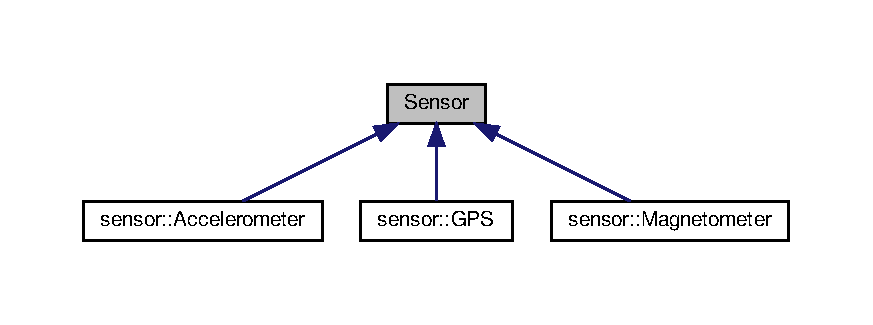
\includegraphics[width=350pt]{class_sensor__inherit__graph}
\end{center}
\end{figure}
\subsection*{Public Member Functions}
\begin{DoxyCompactItemize}
\item 
\hyperlink{class_sensor_a342d6d11ef572c8cba92cb76fb1a294b}{Sensor} ()
\item 
\hyperlink{class_sensor_aa84aad87186b00eb99dd93033bc0cb30}{Sensor} (const std\+::string \&name)
\item 
\hyperlink{class_sensor_aee8c70e7ef05ce65e7ee33686b5d7db2}{$\sim$\+Sensor} ()
\item 
virtual void \hyperlink{class_sensor_a6f16371eb71419f49ea1363ca81d0755}{print\+\_\+raw} ()
\end{DoxyCompactItemize}
\subsection*{Protected Attributes}
\begin{DoxyCompactItemize}
\item 
std\+::string \hyperlink{class_sensor_a364a2c3d5e77d1af61f2532a130c2836}{m\+\_\+name}
\item 
int \hyperlink{class_sensor_a3d1ebe0e05e5d75604330a70d3acf9e5}{m\+\_\+id}
\end{DoxyCompactItemize}
\subsection*{Static Protected Attributes}
\begin{DoxyCompactItemize}
\item 
static int \hyperlink{class_sensor_a67c286c0fd237d5acda6a5b4b99d8aad}{count} = 0
\end{DoxyCompactItemize}


\subsection{Detailed Description}


Definition at line 8 of file sensor.\+h.



\subsection{Constructor \& Destructor Documentation}
\mbox{\Hypertarget{class_sensor_a342d6d11ef572c8cba92cb76fb1a294b}\label{class_sensor_a342d6d11ef572c8cba92cb76fb1a294b}} 
\index{Sensor@{Sensor}!Sensor@{Sensor}}
\index{Sensor@{Sensor}!Sensor@{Sensor}}
\subsubsection{\texorpdfstring{Sensor()}{Sensor()}\hspace{0.1cm}{\footnotesize\ttfamily [1/2]}}
{\footnotesize\ttfamily Sensor\+::\+Sensor (\begin{DoxyParamCaption}{ }\end{DoxyParamCaption})\hspace{0.3cm}{\ttfamily [explicit]}}



Definition at line 4 of file sensor.\+cpp.

\mbox{\Hypertarget{class_sensor_aa84aad87186b00eb99dd93033bc0cb30}\label{class_sensor_aa84aad87186b00eb99dd93033bc0cb30}} 
\index{Sensor@{Sensor}!Sensor@{Sensor}}
\index{Sensor@{Sensor}!Sensor@{Sensor}}
\subsubsection{\texorpdfstring{Sensor()}{Sensor()}\hspace{0.1cm}{\footnotesize\ttfamily [2/2]}}
{\footnotesize\ttfamily Sensor\+::\+Sensor (\begin{DoxyParamCaption}\item[{const std\+::string \&}]{name }\end{DoxyParamCaption})\hspace{0.3cm}{\ttfamily [explicit]}}



Definition at line 8 of file sensor.\+cpp.

\mbox{\Hypertarget{class_sensor_aee8c70e7ef05ce65e7ee33686b5d7db2}\label{class_sensor_aee8c70e7ef05ce65e7ee33686b5d7db2}} 
\index{Sensor@{Sensor}!````~Sensor@{$\sim$\+Sensor}}
\index{````~Sensor@{$\sim$\+Sensor}!Sensor@{Sensor}}
\subsubsection{\texorpdfstring{$\sim$\+Sensor()}{~Sensor()}}
{\footnotesize\ttfamily Sensor\+::$\sim$\+Sensor (\begin{DoxyParamCaption}{ }\end{DoxyParamCaption})}



Definition at line 12 of file sensor.\+cpp.



\subsection{Member Function Documentation}
\mbox{\Hypertarget{class_sensor_a6f16371eb71419f49ea1363ca81d0755}\label{class_sensor_a6f16371eb71419f49ea1363ca81d0755}} 
\index{Sensor@{Sensor}!print\+\_\+raw@{print\+\_\+raw}}
\index{print\+\_\+raw@{print\+\_\+raw}!Sensor@{Sensor}}
\subsubsection{\texorpdfstring{print\+\_\+raw()}{print\_raw()}}
{\footnotesize\ttfamily void Sensor\+::print\+\_\+raw (\begin{DoxyParamCaption}{ }\end{DoxyParamCaption})\hspace{0.3cm}{\ttfamily [virtual]}}



Reimplemented in \hyperlink{classsensor_1_1_g_p_s_a8b0dfe608735ccca47bae8e9a41e1298}{sensor\+::\+G\+PS}, \hyperlink{classsensor_1_1_accelerometer_a172c1bfe5d20071d5f3542a717797afa}{sensor\+::\+Accelerometer}, and \hyperlink{classsensor_1_1_magnetometer_a808eda46aabd080426c909563da0f425}{sensor\+::\+Magnetometer}.



Definition at line 16 of file sensor.\+cpp.



\subsection{Member Data Documentation}
\mbox{\Hypertarget{class_sensor_a67c286c0fd237d5acda6a5b4b99d8aad}\label{class_sensor_a67c286c0fd237d5acda6a5b4b99d8aad}} 
\index{Sensor@{Sensor}!count@{count}}
\index{count@{count}!Sensor@{Sensor}}
\subsubsection{\texorpdfstring{count}{count}}
{\footnotesize\ttfamily int Sensor\+::count = 0\hspace{0.3cm}{\ttfamily [static]}, {\ttfamily [protected]}}



Definition at line 13 of file sensor.\+h.

\mbox{\Hypertarget{class_sensor_a3d1ebe0e05e5d75604330a70d3acf9e5}\label{class_sensor_a3d1ebe0e05e5d75604330a70d3acf9e5}} 
\index{Sensor@{Sensor}!m\+\_\+id@{m\+\_\+id}}
\index{m\+\_\+id@{m\+\_\+id}!Sensor@{Sensor}}
\subsubsection{\texorpdfstring{m\+\_\+id}{m\_id}}
{\footnotesize\ttfamily int Sensor\+::m\+\_\+id\hspace{0.3cm}{\ttfamily [protected]}}



Definition at line 12 of file sensor.\+h.

\mbox{\Hypertarget{class_sensor_a364a2c3d5e77d1af61f2532a130c2836}\label{class_sensor_a364a2c3d5e77d1af61f2532a130c2836}} 
\index{Sensor@{Sensor}!m\+\_\+name@{m\+\_\+name}}
\index{m\+\_\+name@{m\+\_\+name}!Sensor@{Sensor}}
\subsubsection{\texorpdfstring{m\+\_\+name}{m\_name}}
{\footnotesize\ttfamily std\+::string Sensor\+::m\+\_\+name\hspace{0.3cm}{\ttfamily [protected]}}



Definition at line 11 of file sensor.\+h.



The documentation for this class was generated from the following files\+:\begin{DoxyCompactItemize}
\item 
include/\hyperlink{sensor_8h}{sensor.\+h}\item 
src/\hyperlink{sensor_8cpp}{sensor.\+cpp}\end{DoxyCompactItemize}

\chapter{File Documentation}
\hypertarget{accelerometer_8h}{}\section{include/accelerometer.h File Reference}
\label{accelerometer_8h}\index{include/accelerometer.\+h@{include/accelerometer.\+h}}
{\ttfamily \#include $<$vector$>$}\newline
{\ttfamily \#include $<$iostream$>$}\newline
{\ttfamily \#include $<$math.\+h$>$}\newline
{\ttfamily \#include \char`\"{}sensor.\+h\char`\"{}}\newline
{\ttfamily \#include \char`\"{}magnetometer.\+h\char`\"{}}\newline
Include dependency graph for accelerometer.\+h\+:\nopagebreak
\begin{figure}[H]
\begin{center}
\leavevmode
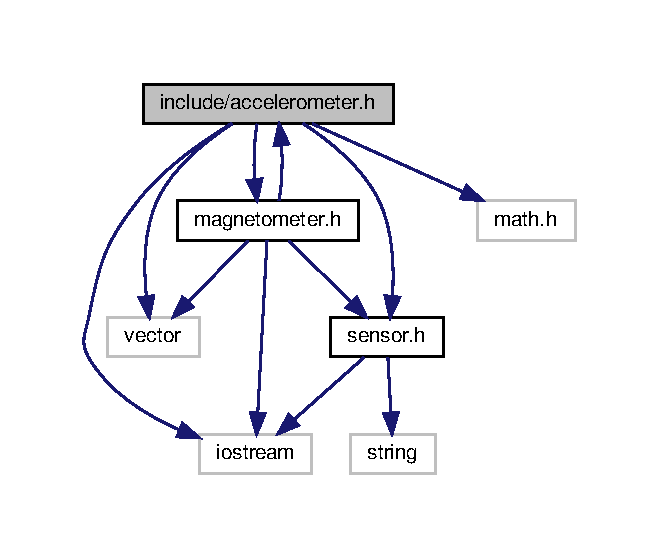
\includegraphics[width=316pt]{accelerometer_8h__incl}
\end{center}
\end{figure}
This graph shows which files directly or indirectly include this file\+:\nopagebreak
\begin{figure}[H]
\begin{center}
\leavevmode
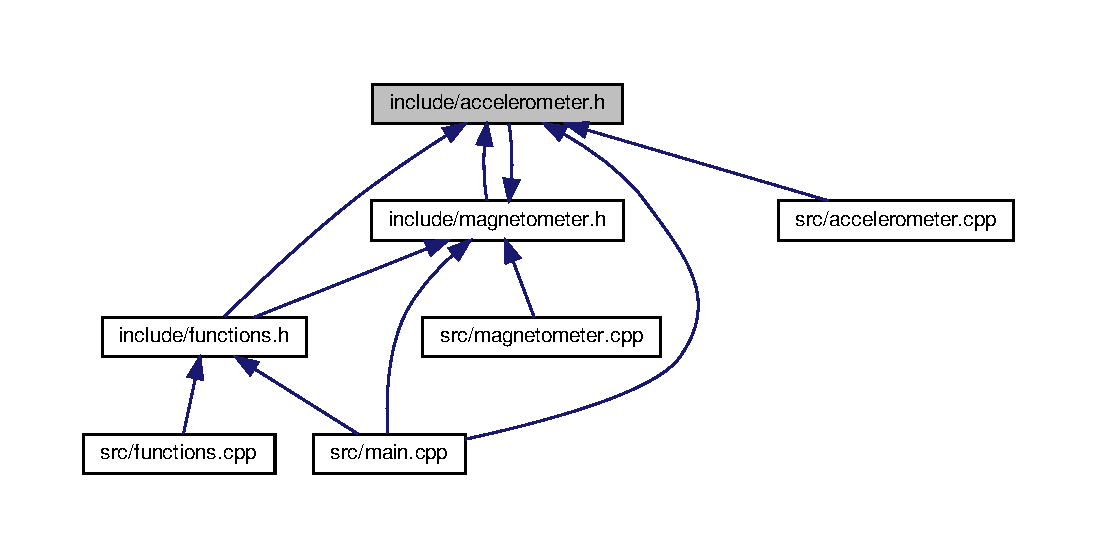
\includegraphics[width=350pt]{accelerometer_8h__dep__incl}
\end{center}
\end{figure}
\subsection*{Classes}
\begin{DoxyCompactItemize}
\item 
class \hyperlink{classsensor_1_1_accelerometer}{sensor\+::\+Accelerometer}
\end{DoxyCompactItemize}
\subsection*{Namespaces}
\begin{DoxyCompactItemize}
\item 
 \hyperlink{namespacesensor}{sensor}
\end{DoxyCompactItemize}
\subsection*{Macros}
\begin{DoxyCompactItemize}
\item 
\#define \hyperlink{accelerometer_8h_aed9ea78689ecce0b7264c02c7f8a9a54}{G}~9.\+81
\item 
\#define \hyperlink{accelerometer_8h_a598a3330b3c21701223ee0ca14316eca}{PI}~3.\+14159265358979323846
\end{DoxyCompactItemize}


\subsection{Macro Definition Documentation}
\mbox{\Hypertarget{accelerometer_8h_aed9ea78689ecce0b7264c02c7f8a9a54}\label{accelerometer_8h_aed9ea78689ecce0b7264c02c7f8a9a54}} 
\index{accelerometer.\+h@{accelerometer.\+h}!G@{G}}
\index{G@{G}!accelerometer.\+h@{accelerometer.\+h}}
\subsubsection{\texorpdfstring{G}{G}}
{\footnotesize\ttfamily \#define G~9.\+81}



Definition at line 10 of file accelerometer.\+h.

\mbox{\Hypertarget{accelerometer_8h_a598a3330b3c21701223ee0ca14316eca}\label{accelerometer_8h_a598a3330b3c21701223ee0ca14316eca}} 
\index{accelerometer.\+h@{accelerometer.\+h}!PI@{PI}}
\index{PI@{PI}!accelerometer.\+h@{accelerometer.\+h}}
\subsubsection{\texorpdfstring{PI}{PI}}
{\footnotesize\ttfamily \#define PI~3.\+14159265358979323846}



Definition at line 11 of file accelerometer.\+h.


\hypertarget{functions_8h}{}\section{include/functions.h File Reference}
\label{functions_8h}\index{include/functions.\+h@{include/functions.\+h}}
{\ttfamily \#include \char`\"{}accelerometer.\+h\char`\"{}}\newline
{\ttfamily \#include \char`\"{}magnetometer.\+h\char`\"{}}\newline
{\ttfamily \#include $<$math.\+h$>$}\newline
{\ttfamily \#include $<$vector$>$}\newline
{\ttfamily \#include $<$iostream$>$}\newline
Include dependency graph for functions.\+h\+:\nopagebreak
\begin{figure}[H]
\begin{center}
\leavevmode
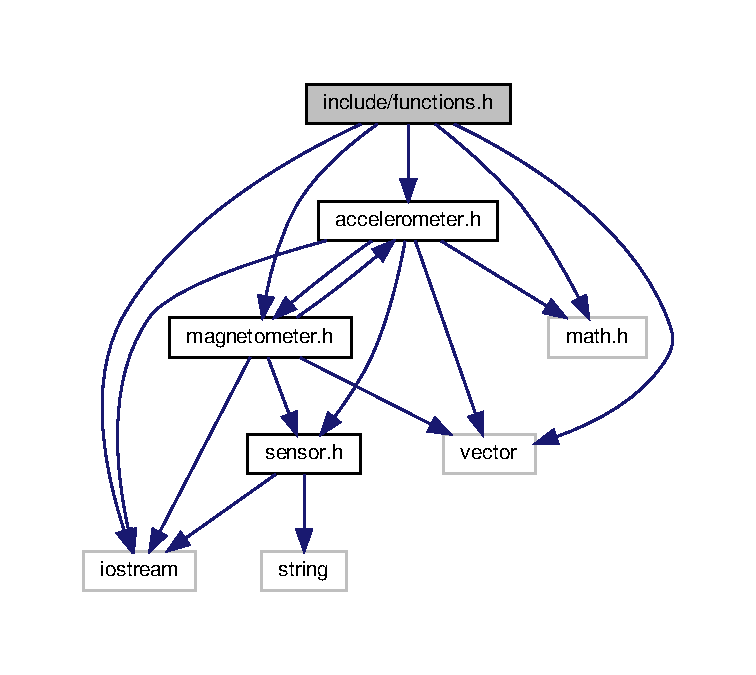
\includegraphics[width=350pt]{functions_8h__incl}
\end{center}
\end{figure}
This graph shows which files directly or indirectly include this file\+:\nopagebreak
\begin{figure}[H]
\begin{center}
\leavevmode
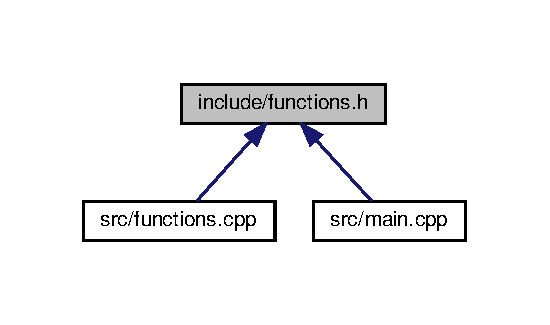
\includegraphics[width=264pt]{functions_8h__dep__incl}
\end{center}
\end{figure}
\subsection*{Namespaces}
\begin{DoxyCompactItemize}
\item 
 \hyperlink{namespacesensor}{sensor}
\end{DoxyCompactItemize}
\subsection*{Functions}
\begin{DoxyCompactItemize}
\item 
std\+::vector$<$ double $>$ \hyperlink{namespacesensor_a8d403ba02d81030a8c321487632d6dfd}{sensor\+::\+Roll\+Pitch\+Yaw} (Accelerometer \&obj\+\_\+acc, Magnetometer \&obj\+\_\+mag)
\end{DoxyCompactItemize}

\hypertarget{gps_8h}{}\section{include/gps.h File Reference}
\label{gps_8h}\index{include/gps.\+h@{include/gps.\+h}}
{\ttfamily \#include $<$iostream$>$}\newline
{\ttfamily \#include $<$vector$>$}\newline
{\ttfamily \#include $<$string$>$}\newline
{\ttfamily \#include \char`\"{}sensor.\+h\char`\"{}}\newline
{\ttfamily \#include $<$math.\+h$>$}\newline
Include dependency graph for gps.\+h\+:\nopagebreak
\begin{figure}[H]
\begin{center}
\leavevmode
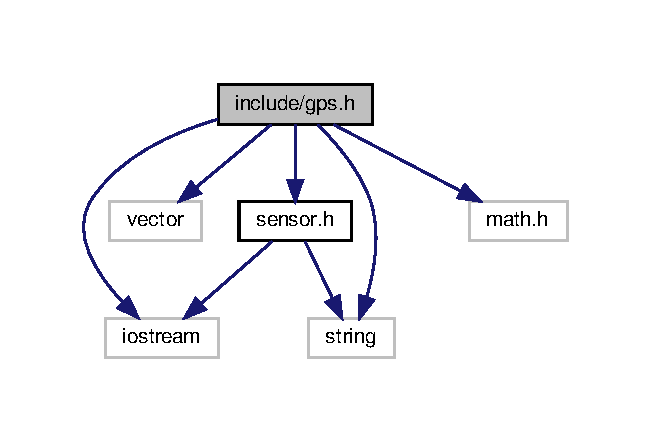
\includegraphics[width=312pt]{gps_8h__incl}
\end{center}
\end{figure}
This graph shows which files directly or indirectly include this file\+:\nopagebreak
\begin{figure}[H]
\begin{center}
\leavevmode
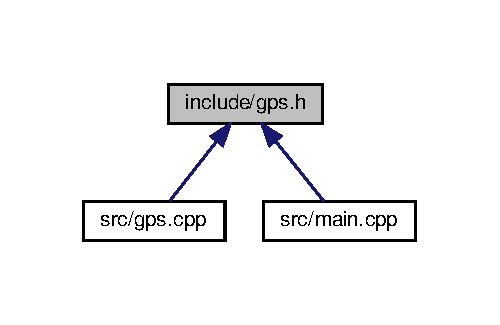
\includegraphics[width=240pt]{gps_8h__dep__incl}
\end{center}
\end{figure}
\subsection*{Classes}
\begin{DoxyCompactItemize}
\item 
class \hyperlink{classsensor_1_1_g_p_s}{sensor\+::\+G\+PS}
\end{DoxyCompactItemize}
\subsection*{Namespaces}
\begin{DoxyCompactItemize}
\item 
 \hyperlink{namespacesensor}{sensor}
\end{DoxyCompactItemize}
\subsection*{Macros}
\begin{DoxyCompactItemize}
\item 
\#define \hyperlink{gps_8h_aed9ea78689ecce0b7264c02c7f8a9a54}{G}~9.\+81
\item 
\#define \hyperlink{gps_8h_a598a3330b3c21701223ee0ca14316eca}{PI}~3.\+14159265358979323846
\end{DoxyCompactItemize}


\subsection{Macro Definition Documentation}
\mbox{\Hypertarget{gps_8h_aed9ea78689ecce0b7264c02c7f8a9a54}\label{gps_8h_aed9ea78689ecce0b7264c02c7f8a9a54}} 
\index{gps.\+h@{gps.\+h}!G@{G}}
\index{G@{G}!gps.\+h@{gps.\+h}}
\subsubsection{\texorpdfstring{G}{G}}
{\footnotesize\ttfamily \#define G~9.\+81}



Definition at line 10 of file gps.\+h.

\mbox{\Hypertarget{gps_8h_a598a3330b3c21701223ee0ca14316eca}\label{gps_8h_a598a3330b3c21701223ee0ca14316eca}} 
\index{gps.\+h@{gps.\+h}!PI@{PI}}
\index{PI@{PI}!gps.\+h@{gps.\+h}}
\subsubsection{\texorpdfstring{PI}{PI}}
{\footnotesize\ttfamily \#define PI~3.\+14159265358979323846}



Definition at line 11 of file gps.\+h.


\hypertarget{magnetometer_8h}{}\section{include/magnetometer.h File Reference}
\label{magnetometer_8h}\index{include/magnetometer.\+h@{include/magnetometer.\+h}}
{\ttfamily \#include $<$iostream$>$}\newline
{\ttfamily \#include $<$vector$>$}\newline
{\ttfamily \#include \char`\"{}accelerometer.\+h\char`\"{}}\newline
{\ttfamily \#include \char`\"{}sensor.\+h\char`\"{}}\newline
Include dependency graph for magnetometer.\+h\+:\nopagebreak
\begin{figure}[H]
\begin{center}
\leavevmode
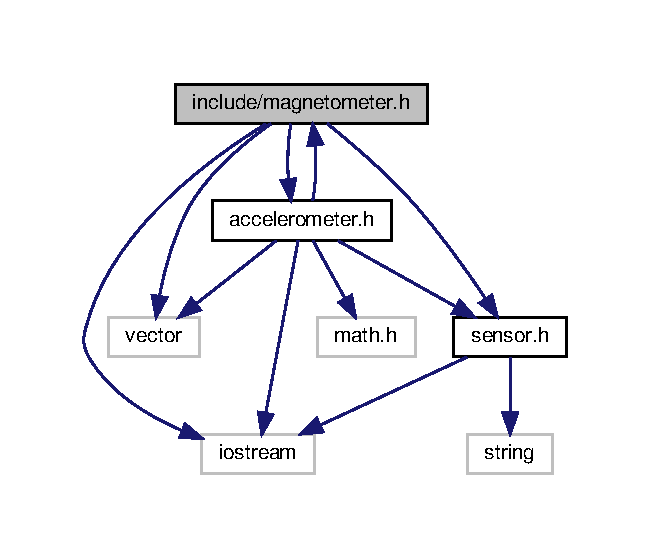
\includegraphics[width=312pt]{magnetometer_8h__incl}
\end{center}
\end{figure}
This graph shows which files directly or indirectly include this file\+:\nopagebreak
\begin{figure}[H]
\begin{center}
\leavevmode
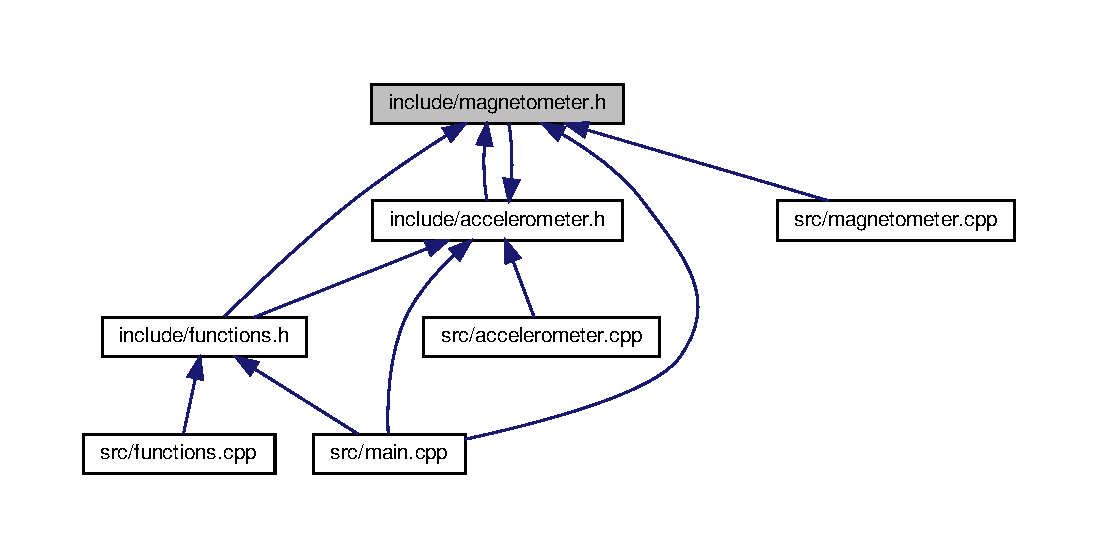
\includegraphics[width=350pt]{magnetometer_8h__dep__incl}
\end{center}
\end{figure}
\subsection*{Classes}
\begin{DoxyCompactItemize}
\item 
class \hyperlink{classsensor_1_1_magnetometer}{sensor\+::\+Magnetometer}
\end{DoxyCompactItemize}
\subsection*{Namespaces}
\begin{DoxyCompactItemize}
\item 
 \hyperlink{namespacesensor}{sensor}
\end{DoxyCompactItemize}

\hypertarget{sensor_8h}{}\section{include/sensor.h File Reference}
\label{sensor_8h}\index{include/sensor.\+h@{include/sensor.\+h}}
{\ttfamily \#include $<$string$>$}\newline
{\ttfamily \#include $<$iostream$>$}\newline
Include dependency graph for sensor.\+h\+:\nopagebreak
\begin{figure}[H]
\begin{center}
\leavevmode
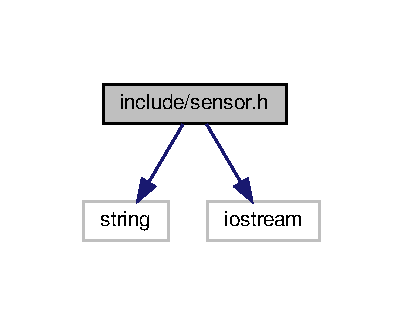
\includegraphics[width=194pt]{sensor_8h__incl}
\end{center}
\end{figure}
This graph shows which files directly or indirectly include this file\+:\nopagebreak
\begin{figure}[H]
\begin{center}
\leavevmode
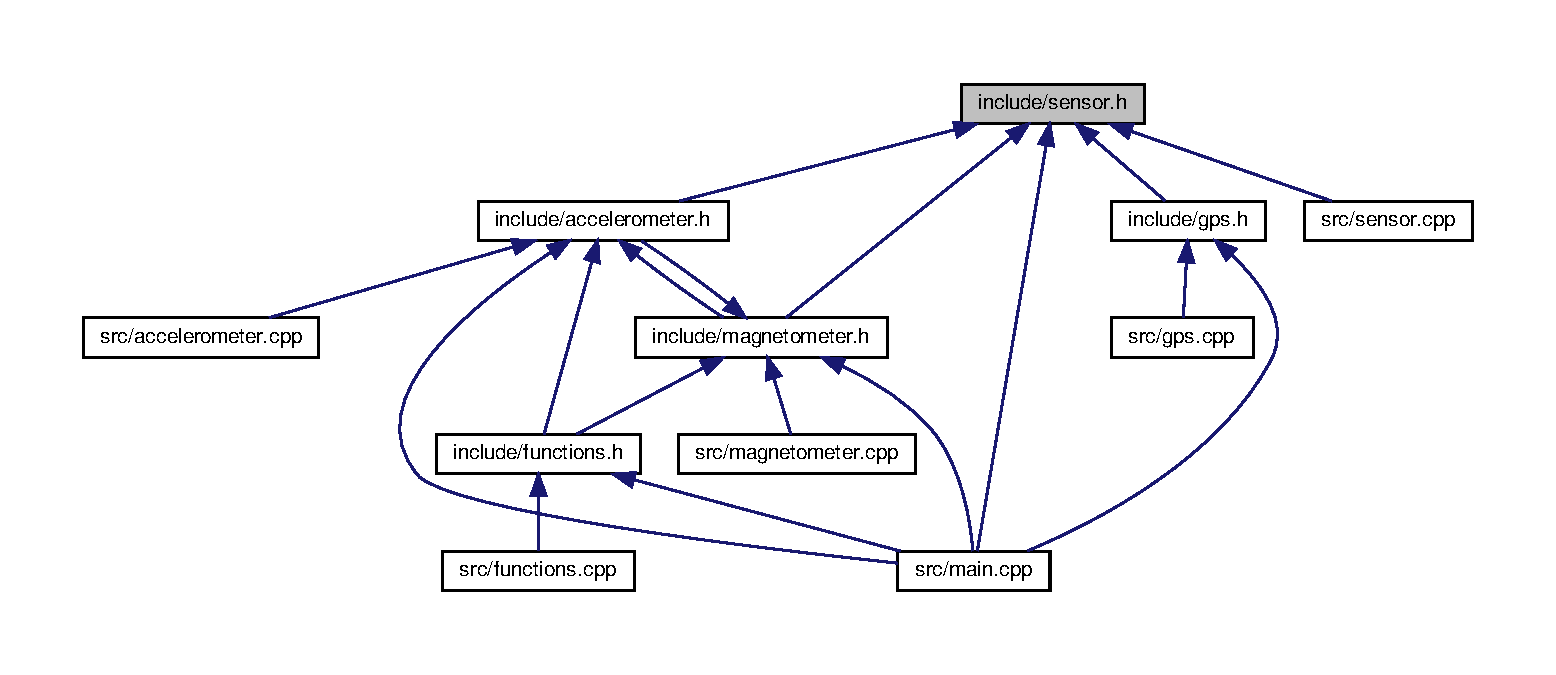
\includegraphics[width=350pt]{sensor_8h__dep__incl}
\end{center}
\end{figure}
\subsection*{Classes}
\begin{DoxyCompactItemize}
\item 
class \hyperlink{class_sensor}{Sensor}
\end{DoxyCompactItemize}

\hypertarget{accelerometer_8cpp}{}\section{src/accelerometer.cpp File Reference}
\label{accelerometer_8cpp}\index{src/accelerometer.\+cpp@{src/accelerometer.\+cpp}}
{\ttfamily \#include \char`\"{}include/accelerometer.\+h\char`\"{}}\newline
Include dependency graph for accelerometer.\+cpp\+:\nopagebreak
\begin{figure}[H]
\begin{center}
\leavevmode
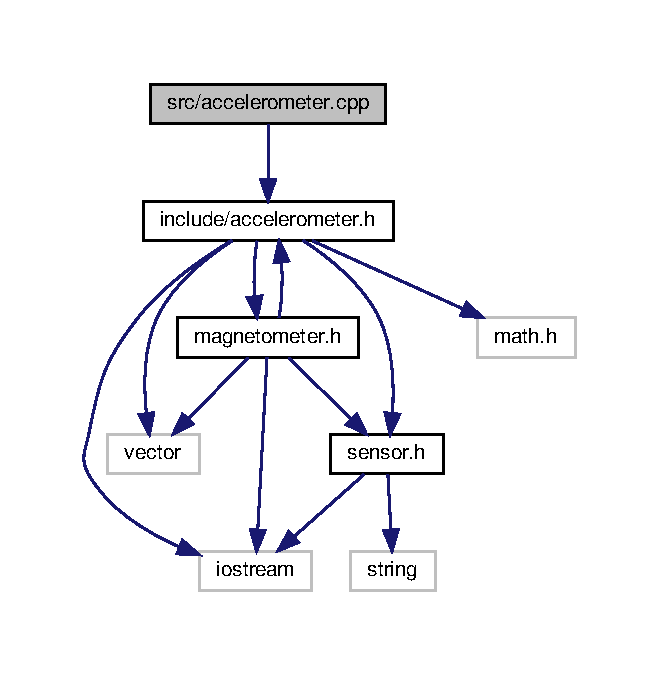
\includegraphics[width=316pt]{accelerometer_8cpp__incl}
\end{center}
\end{figure}
\subsection*{Namespaces}
\begin{DoxyCompactItemize}
\item 
 \hyperlink{namespacesensor}{sensor}
\end{DoxyCompactItemize}

\hypertarget{functions_8cpp}{}\section{src/functions.cpp File Reference}
\label{functions_8cpp}\index{src/functions.\+cpp@{src/functions.\+cpp}}
{\ttfamily \#include \char`\"{}include/functions.\+h\char`\"{}}\newline
Include dependency graph for functions.\+cpp\+:\nopagebreak
\begin{figure}[H]
\begin{center}
\leavevmode
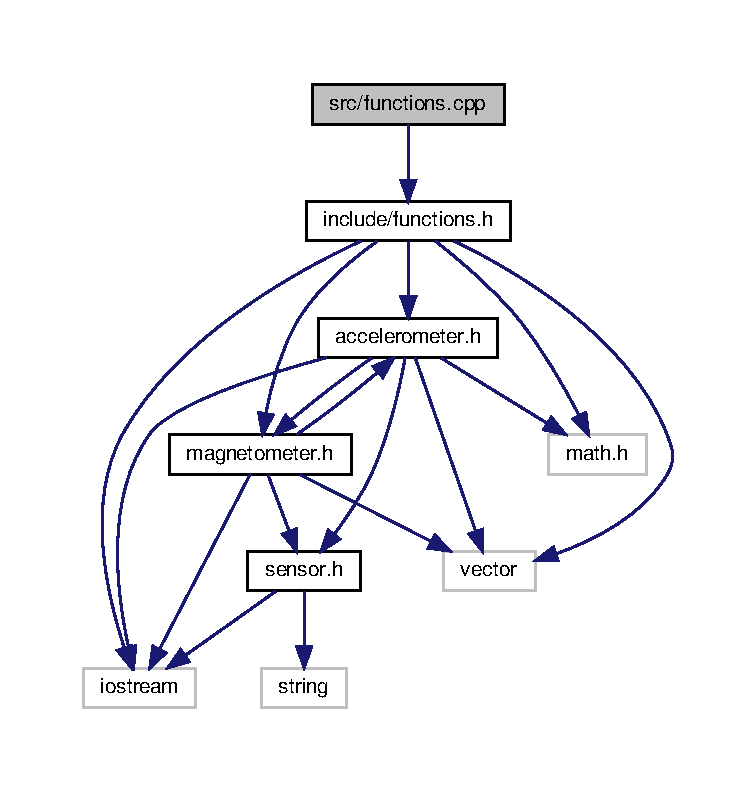
\includegraphics[width=350pt]{functions_8cpp__incl}
\end{center}
\end{figure}
\subsection*{Namespaces}
\begin{DoxyCompactItemize}
\item 
 \hyperlink{namespacesensor}{sensor}
\end{DoxyCompactItemize}
\subsection*{Functions}
\begin{DoxyCompactItemize}
\item 
std\+::vector$<$ double $>$ \hyperlink{namespacesensor_a8d403ba02d81030a8c321487632d6dfd}{sensor\+::\+Roll\+Pitch\+Yaw} (Accelerometer \&obj\+\_\+acc, Magnetometer \&obj\+\_\+mag)
\end{DoxyCompactItemize}

\hypertarget{gps_8cpp}{}\section{src/gps.cpp File Reference}
\label{gps_8cpp}\index{src/gps.\+cpp@{src/gps.\+cpp}}
{\ttfamily \#include \char`\"{}include/gps.\+h\char`\"{}}\newline
Include dependency graph for gps.\+cpp\+:\nopagebreak
\begin{figure}[H]
\begin{center}
\leavevmode
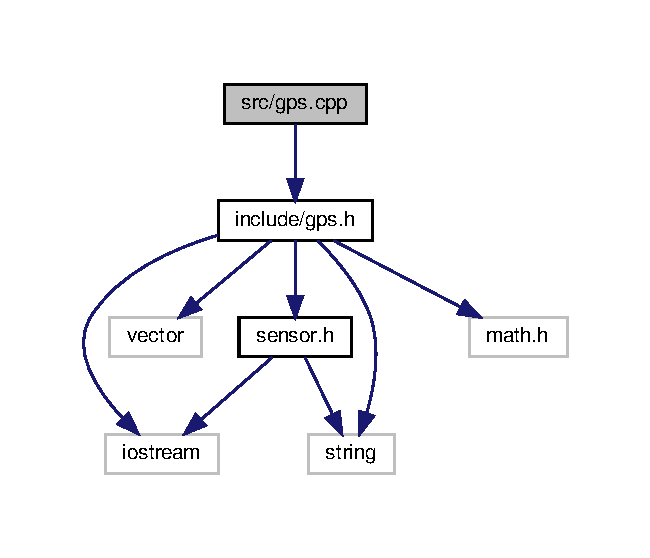
\includegraphics[width=312pt]{gps_8cpp__incl}
\end{center}
\end{figure}
\subsection*{Namespaces}
\begin{DoxyCompactItemize}
\item 
 \hyperlink{namespacesensor}{sensor}
\end{DoxyCompactItemize}

\hypertarget{magnetometer_8cpp}{}\section{src/magnetometer.cpp File Reference}
\label{magnetometer_8cpp}\index{src/magnetometer.\+cpp@{src/magnetometer.\+cpp}}
{\ttfamily \#include \char`\"{}include/magnetometer.\+h\char`\"{}}\newline
Include dependency graph for magnetometer.\+cpp\+:\nopagebreak
\begin{figure}[H]
\begin{center}
\leavevmode
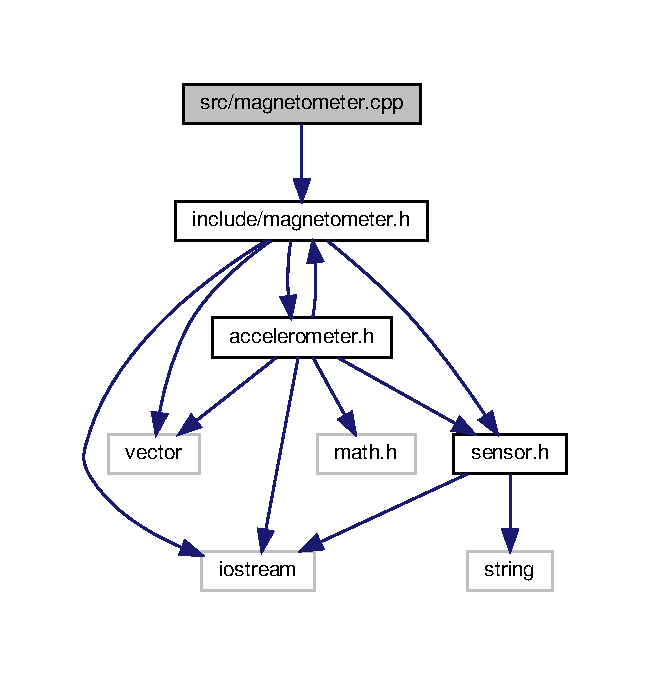
\includegraphics[width=312pt]{magnetometer_8cpp__incl}
\end{center}
\end{figure}
\subsection*{Namespaces}
\begin{DoxyCompactItemize}
\item 
 \hyperlink{namespacesensor}{sensor}
\end{DoxyCompactItemize}

\hypertarget{main_8cpp}{}\section{src/main.cpp File Reference}
\label{main_8cpp}\index{src/main.\+cpp@{src/main.\+cpp}}
{\ttfamily \#include $<$fstream$>$}\newline
{\ttfamily \#include $<$iostream$>$}\newline
{\ttfamily \#include \char`\"{}include/sensor.\+h\char`\"{}}\newline
{\ttfamily \#include \char`\"{}include/accelerometer.\+h\char`\"{}}\newline
{\ttfamily \#include \char`\"{}include/magnetometer.\+h\char`\"{}}\newline
{\ttfamily \#include \char`\"{}include/functions.\+h\char`\"{}}\newline
{\ttfamily \#include \char`\"{}include/gps.\+h\char`\"{}}\newline
{\ttfamily \#include \char`\"{}include/json.\+hpp\char`\"{}}\newline
Include dependency graph for main.\+cpp\+:
\nopagebreak
\begin{figure}[H]
\begin{center}
\leavevmode
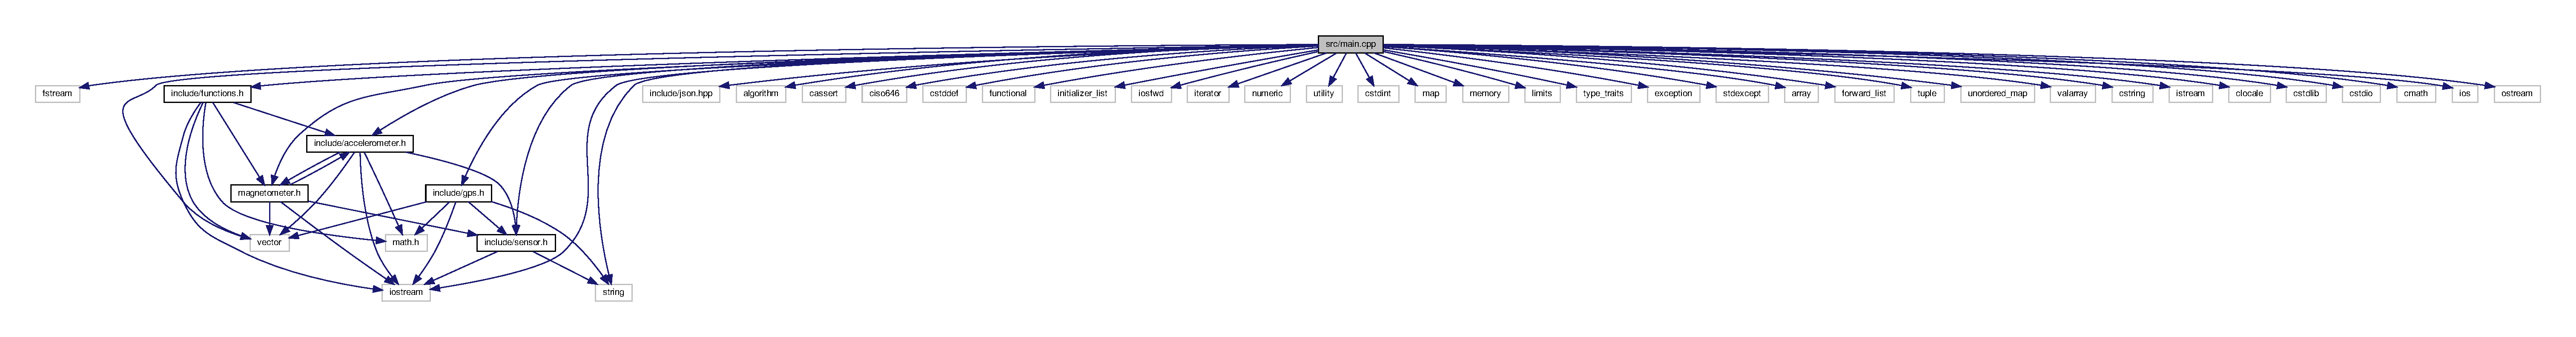
\includegraphics[width=350pt]{main_8cpp__incl}
\end{center}
\end{figure}
\subsection*{Macros}
\begin{DoxyCompactItemize}
\item 
\#define \hyperlink{main_8cpp_aed9ea78689ecce0b7264c02c7f8a9a54}{G}~9.\+81
\item 
\#define \hyperlink{main_8cpp_a598a3330b3c21701223ee0ca14316eca}{PI}~3.\+14159265358979323846
\end{DoxyCompactItemize}
\subsection*{Functions}
\begin{DoxyCompactItemize}
\item 
int \hyperlink{main_8cpp_ae66f6b31b5ad750f1fe042a706a4e3d4}{main} ()
\end{DoxyCompactItemize}


\subsection{Macro Definition Documentation}
\mbox{\Hypertarget{main_8cpp_aed9ea78689ecce0b7264c02c7f8a9a54}\label{main_8cpp_aed9ea78689ecce0b7264c02c7f8a9a54}} 
\index{main.\+cpp@{main.\+cpp}!G@{G}}
\index{G@{G}!main.\+cpp@{main.\+cpp}}
\subsubsection{\texorpdfstring{G}{G}}
{\footnotesize\ttfamily \#define G~9.\+81}



Definition at line 12 of file main.\+cpp.

\mbox{\Hypertarget{main_8cpp_a598a3330b3c21701223ee0ca14316eca}\label{main_8cpp_a598a3330b3c21701223ee0ca14316eca}} 
\index{main.\+cpp@{main.\+cpp}!PI@{PI}}
\index{PI@{PI}!main.\+cpp@{main.\+cpp}}
\subsubsection{\texorpdfstring{PI}{PI}}
{\footnotesize\ttfamily \#define PI~3.\+14159265358979323846}



Definition at line 13 of file main.\+cpp.



\subsection{Function Documentation}
\mbox{\Hypertarget{main_8cpp_ae66f6b31b5ad750f1fe042a706a4e3d4}\label{main_8cpp_ae66f6b31b5ad750f1fe042a706a4e3d4}} 
\index{main.\+cpp@{main.\+cpp}!main@{main}}
\index{main@{main}!main.\+cpp@{main.\+cpp}}
\subsubsection{\texorpdfstring{main()}{main()}}
{\footnotesize\ttfamily int main (\begin{DoxyParamCaption}{ }\end{DoxyParamCaption})}



Definition at line 15 of file main.\+cpp.


\hypertarget{sensor_8cpp}{}\section{src/sensor.cpp File Reference}
\label{sensor_8cpp}\index{src/sensor.\+cpp@{src/sensor.\+cpp}}
{\ttfamily \#include \char`\"{}include/sensor.\+h\char`\"{}}\newline
Include dependency graph for sensor.\+cpp\+:\nopagebreak
\begin{figure}[H]
\begin{center}
\leavevmode
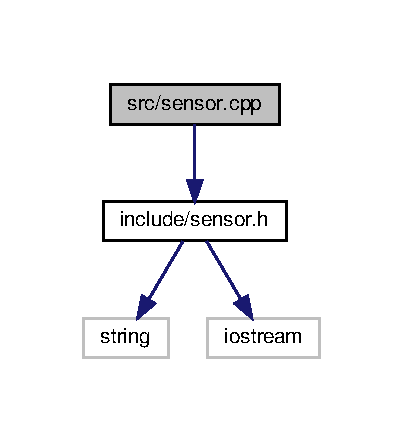
\includegraphics[width=194pt]{sensor_8cpp__incl}
\end{center}
\end{figure}

%--- End generated contents ---

% Index
\backmatter
\newpage
\phantomsection
\clearemptydoublepage
\addcontentsline{toc}{chapter}{Index}
\printindex

\end{document}
